\documentclass[a4paper,14pt]{extarticle}

\usepackage[utf8x]{inputenc}
\usepackage[T1]{fontenc}
\usepackage[russian]{babel}
\usepackage{hyperref}
\usepackage{indentfirst}
\usepackage{here}
\usepackage{array}
\usepackage{graphicx}
\usepackage{grffile}
\usepackage{caption}
\usepackage{subcaption}
\usepackage{chngcntr}
\usepackage{amsmath}
\usepackage{amssymb}
\usepackage{pgfplots}
\usepackage{pgfplotstable}
\usepackage[left=2cm,right=2cm,top=2cm,bottom=2cm,bindingoffset=0cm]{geometry}
\usepackage{multicol}
\usepackage{multirow}
\usepackage{titlesec}
\usepackage{listings}
\usepackage{color}
\usepackage{longtable}
\usepackage{enumitem}
\usepackage{cmap}
\usepackage{tikz}

\usetikzlibrary{shapes,arrows}

\definecolor{green}{rgb}{0,0.6,0}
\definecolor{gray}{rgb}{0.5,0.5,0.5}
\definecolor{purple}{rgb}{0.58,0,0.82}

\lstset{
	language={SQL},
	inputpath={../},
	backgroundcolor=\color{white},
	commentstyle=\color{green},
	keywordstyle=\color{blue},
	numberstyle=\scriptsize\color{gray},
	stringstyle=\color{purple},
	basicstyle=\small,
	breakatwhitespace=false,
	breaklines=true,
	captionpos=b,
	keepspaces=true,
	numbers=left,
	numbersep=5pt,
	showspaces=false,
	showstringspaces=false,
	showtabs=false,
	tabsize=8,
	frame=single,
}

\renewcommand{\le}{\ensuremath{\leqslant}}
\renewcommand{\leq}{\ensuremath{\leqslant}}
\renewcommand{\ge}{\ensuremath{\geqslant}}
\renewcommand{\geq}{\ensuremath{\geqslant}}
\renewcommand{\epsilon}{\ensuremath{\varepsilon}}
\renewcommand{\phi}{\ensuremath{\varphi}}
\renewcommand{\thefigure}{\arabic{figure}}
\def\code#1{\texttt{#1}}

\titleformat*{\section}{\large\bfseries} 
\titleformat*{\subsection}{\normalsize\bfseries} 
\titleformat*{\subsubsection}{\normalsize\bfseries} 
\titleformat*{\paragraph}{\normalsize\bfseries} 
\titleformat*{\subparagraph}{\normalsize\bfseries} 

\counterwithin{figure}{section}
\counterwithin{equation}{section}
\counterwithin{table}{section}
\newcommand{\sign}[1][5cm]{\makebox[#1]{\hrulefill}}
\newcommand{\equipollence}{\quad\Leftrightarrow\quad}
\newcommand{\no}[1]{\overline{#1}}
\graphicspath{{../}}
\captionsetup{justification=centering,margin=1cm}
\def\arraystretch{1.3}
\setlength\parindent{5ex}
\titlelabel{\thetitle.\quad}

\setitemize{itemsep=0em}
\setenumerate{itemsep=0em}

\tikzstyle{startstop} = [
	rectangle,
	align=center,
	rounded corners,
	text width=10em,
	text centered,
	draw=black
]
\tikzstyle{process} = [
	rectangle,
	align=center,
	text width=20em,
	text centered,
	draw=black
]
\tikzstyle{decision} = [
	diamond,
	aspect=4,
	align=center,
	inner sep=0pt,
	text width=10em,
	text centered,
	node distance=5em,
	draw=black
]
\tikzstyle{line} = [
	draw=black,
	thick,
	->,
	>=stealth,
	-latex'
]

\begin{document}

\begin{titlepage}
\begin{center}
	САНКТ-ПЕТЕРБУРГСКИЙ ПОЛИТЕХНИЧЕСКИЙ УНИВЕРСИТЕТ\\ ПЕТРА ВЕЛИКОГО\\[0.3cm]
	\par\noindent\rule{10cm}{0.4pt}\\[0.3cm]
	Институт компьютерных наук и технологий \\[0.3cm]
	Кафедра компьютерных систем и программных технологий\\[4cm]
	
	Отчет по лабораторной работе № 1\\[3mm]
	Дисциплина: <<Базы данных>>\\[3mm]
	Тема: <<Разработка структуры БД>>\\[7cm]
\end{center}

\begin{flushleft}
	\hspace*{5mm} Выполнил студент гр. 43501/3  \hspace*{2.5cm}\sign[3cm]\hspace*{3.0mm} А.Ю. Ламтев\\
	\hspace*{10.4cm} (подпись)\\[3mm]
	\hspace*{5mm} Преподаватель \hspace*{6.0cm}\sign[3cm]\hspace*{2mm} А.В. Мяснов\\
	\hspace*{10.4cm} (подпись)\\[3mm]
	\hspace*{11.1cm} <<\sign[7mm]>> \sign[27mm] \the\year\hspace{1mm} г.
\end{flushleft}

\vfill

\begin{center}
	Санкт-Петербург\\
	\the\year
\end{center}
\end{titlepage}
\addtocounter{page}{1}

\tableofcontents
\newpage

\section{Цели работы}

Познакомитьcя с языком создания запросов управления данными SQL DML. 

\section{Программа работы}

\begin{enumerate}
	\item Изучение SQL DML.
	\item Выполнение всех запросов из списка стандартных запросов. Демонстрация результатов преподавателю.
	\item Получение у преподавателя и реализация SQL-запросов в соответствии с индивидуальным заданием. 			\item Демонстрация результатов преподавателю.
	\item Сохранение в БД выполненных запросов \code{SELECT} в виде представлений, запросов \code{INSERT}, \code{UPDATE} или \code{DELETE} --- в виде ХП.
 
\end{enumerate}
 
\section{Стандартные запросы} 

\subsection{Выборка данных из одной таблицы с использованием логических операций, \code{LIKE}, \code{BETWEEN}, \code{IN}}

В листинге \ref{lst:like-between-in-1.sql} представлен запрос, формирующий выборку пользователей мужского пола, родившихся до 30 декабря 2001 года, и длина логина которых находится в диапазоне между 7 и 11.

\lstinputlisting[caption={like-between-in-1.sql},label={lst:like-between-in-1.sql}]{like-between-in-1.sql}
 
Выборка, сформированная данным запросом, представлена на рис. \ref{fig:like-between-in-1}.

\begin{figure}[H]
	\centering
	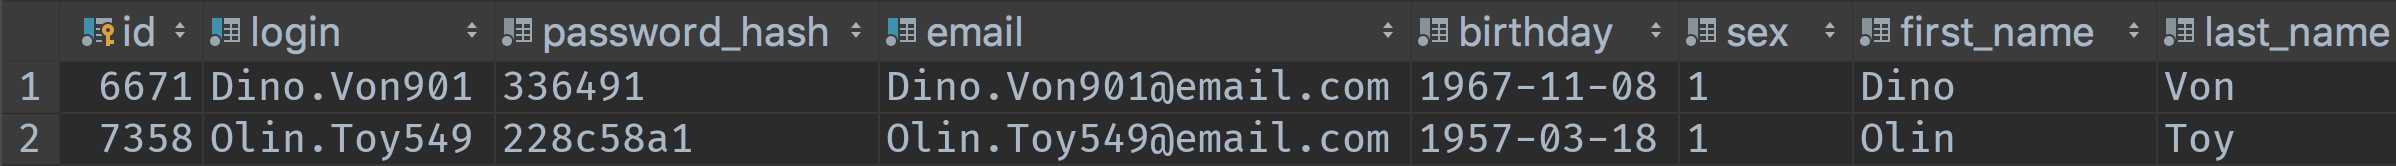
\includegraphics[width=1.0\textwidth]{like-between-in-1.png}
	\caption{Выборка, сформированная \code{like-between-in-1.sql}}
	\label{fig:like-between-in-1}
\end{figure}
 

В листинге \ref{lst:like-between-in-2.sql} представлен запрос, формирующий выборку пользователей женского пола, логин которых начинается с <<\code{Marie.}>>.

\lstinputlisting[caption={like-between-in-2.sql},label={lst:like-between-in-2.sql}]{like-between-in-2.sql}

Выборка, сформированная данным запросом, представлена на рис. \ref{fig:like-between-in-2}.

\begin{figure}[H]
	\centering
	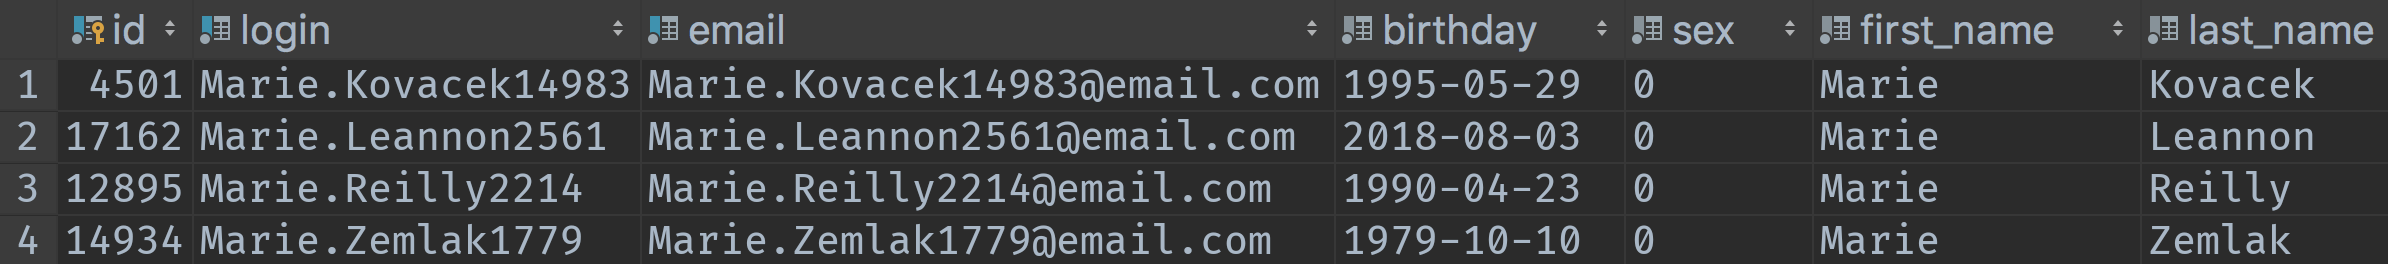
\includegraphics[width=1.0\textwidth]{like-between-in-2.png}
	\caption{Выборка, сформированная \code{like-between-in-2.sql}}
	\label{fig:like-between-in-2}
\end{figure}

В листинге \ref{lst:like-between-in-3.sql} представлен запрос, формирующий выборку фильмов, цена которых \$$5$ или \$$7$, при этом они не являются эпизодами сериалов, они были выпущены в октябре (не важно какого года), и их \code{IMDB} рэйтинг лежит в диапазоне между $7.5$ и $7.6$. Поля выборки следующие: идентификатор, стоимость, возраст в годах и рейтинг \code{IMDB}.

\lstinputlisting[caption={like-between-in-3.sql},label={lst:like-between-in-3.sql}]{like-between-in-3.sql}

Выборка, сформированная данным запросом, представлена на рис. \ref{fig:like-between-in-3}.

\begin{figure}[H]
	\centering
	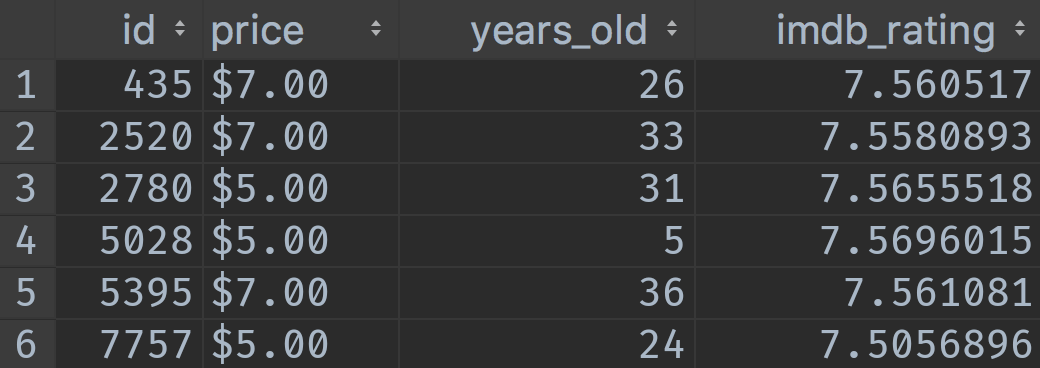
\includegraphics[width=0.4\textwidth]{like-between-in-3.png}
	\caption{Выборка, сформированная \code{like-between-in-3.sql}}
	\label{fig:like-between-in-3}
\end{figure}

\subsection{Запрос с вычисляемым полем}

В листинге \ref{lst:calculated-field.sql} представлен запрос, формирующий выборку из 5-ти еще не закончившихся, автоматически возобновляемых подписок, длительность которых равна 30 дням. Поля у выборки следующие: идентификатор подписки, идентификатор пользователя, стоимость и число дней до завершения подписки. При этом последнее поле является вычисляемым.

\lstinputlisting[caption={calculated-field.sql},label={lst:calculated-field.sql}]{calculated-field.sql}

Выборка, сформированная данным запросом, представлена на рис. \ref{fig:calculated-field}.

\begin{figure}[H]
	\centering
	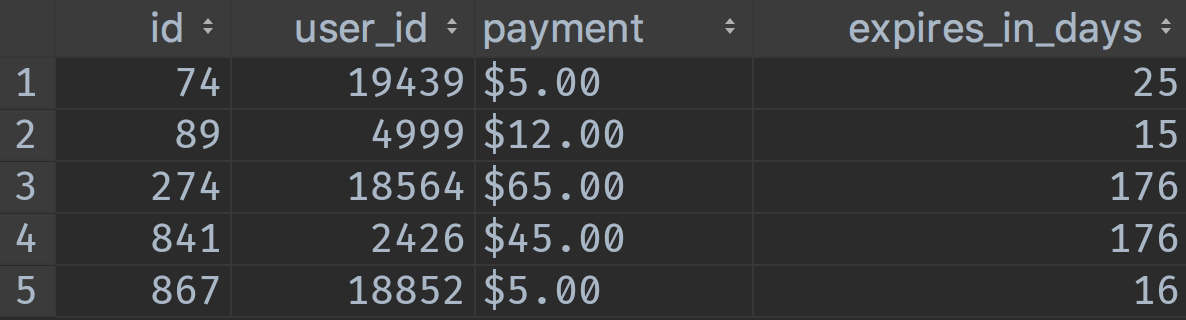
\includegraphics[width=0.45\textwidth]{calculated-field.png}
	\caption{Выборка, сформированная \code{calculated-field.sql}}
	\label{fig:calculated-field}
\end{figure}

Значения в столбце \code{expires\_in\_days}, превосходящие 30, объясняются тем, что эти подписки еще не вступили в силу.

\subsection{Выборка с сортировкой по нескольким полям}

В листинге \ref{lst:sorted.sql} представлен запрос, формирующий выборку из 5-ти сериалов, при этом сериалы отсортированы по возрастанию числа сезонов и по убыванию стоимости.

\lstinputlisting[caption={sorted.sql},label={lst:sorted.sql}]{sorted.sql}

Выборка, сформированная данным запросом, представлена на рис. \ref{fig:sorted}.

\begin{figure}[H]
	\centering
	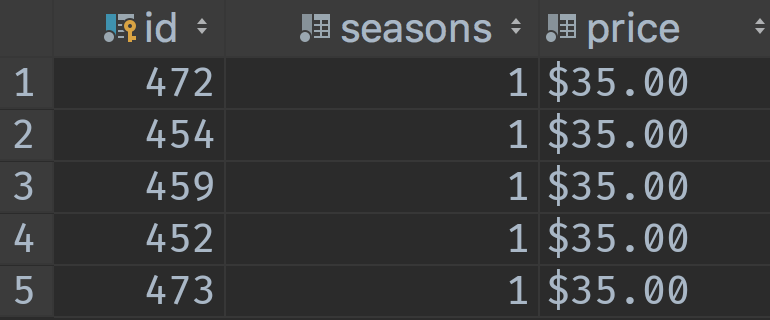
\includegraphics[width=0.32\textwidth]{sorted.png}
	\caption{Выборка, сформированная \code{sorted.sql}}
	\label{fig:sorted}
\end{figure}

\subsection{Запрос с вычислением совокупных характеристик}

В листинге \ref{lst:aggregate.sql} представлен запрос, формирующий одну строку, содержащую общее число пользователей, максимальную длину имени, минимальную длину фамилии, средний возраст пользователей, а также число ползователей мужского пола.

\lstinputlisting[caption={aggregate.sql},label={lst:aggregate.sql}]{aggregate.sql}

Выборка, сформированная данным запросом, представлена на рис. \ref{fig:aggregate}.

\begin{figure}[H]
	\centering
	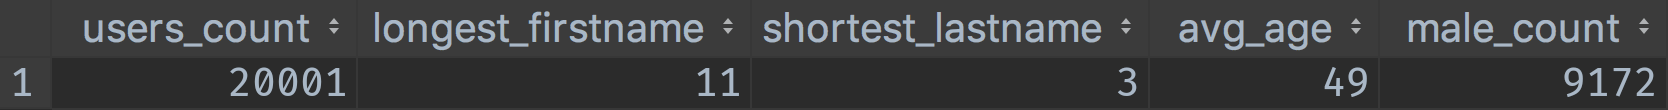
\includegraphics[width=0.8\textwidth]{aggregate.png}
	\caption{Выборка, сформированная \code{aggregate.sql}}
	\label{fig:aggregate}
\end{figure}

\subsection{Выборка данных из связанных таблиц}

В листинге \ref{lst:join1.sql} представлен запрос, в котором соединяются 2 таблицы --- \code{series} (сериалы) и \code{series\_translation} (переводы сериалов) для формирования названия сериала с наибольшим числом сезонов и наибольшей стоимостью.

\lstinputlisting[caption={join1.sql},label={lst:join1.sql}]{join1.sql}

Выборка, сформированная данным запросом, представлена на рис. \ref{fig:join1}.

\begin{figure}[H]
	\centering
	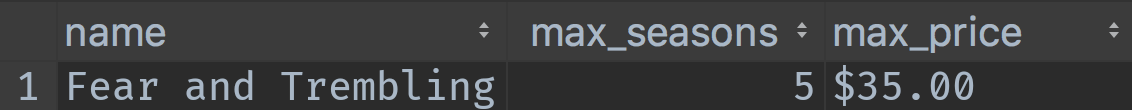
\includegraphics[width=0.5\textwidth]{join1.png}
	\caption{Выборка, сформированная \code{join1.sql}}
	\label{fig:join1}
\end{figure}

В листинге \ref{lst:join2.sql} представлен запрос, в котором соединяются 3 таблицы --- \code{movie\_translation} (переводы фильмов), \code{language} (языки) и \code{user\_movie} (пользователи -- фильмы) для определения наиболее часто приобретаемого фильма, который не является эпизодом сериала. Выборка состоит из 2-х записей, содержащих идентификатор фильма, имя фильма, локаль и частоту его покупки, для 2-х локалей: русской и английской.

\lstinputlisting[caption={join2.sql},label={lst:join2.sql}]{join2.sql}

Выборка, сформированная данным запросом, представлена на рис. \ref{fig:join2}.

\begin{figure}[H]
	\centering
	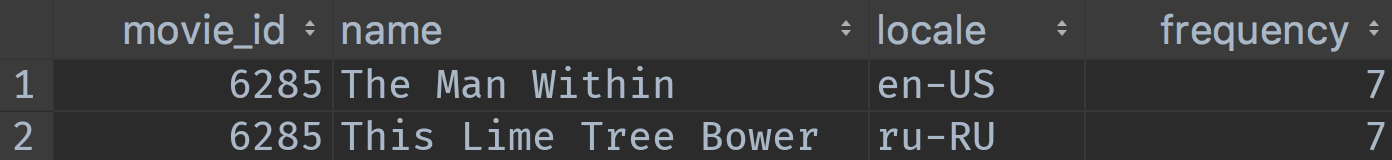
\includegraphics[width=0.5\textwidth]{join2.png}
	\caption{Выборка, сформированная \code{join2.sql}}
	\label{fig:join2}
\end{figure}

\subsection{Запрос с подзапросами}

В листинге \ref{lst:inner.sql} представлен запрос, который аналогично предыдущему запросу выводит название фильма, который наиболее часто покупается пользователями, но уже с помощью вложенных подзапросов.
\lstinputlisting[caption={inner.sql},label={lst:inner.sql}]{inner.sql}

Выборка, сформированная данным запросом, представлена на рис. \ref{fig:inner}.

\begin{figure}[H]
	\centering
	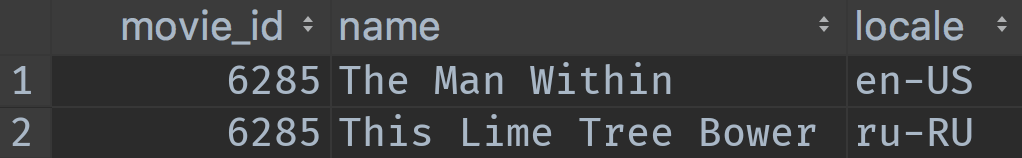
\includegraphics[width=0.4\textwidth]{inner.png}
	\caption{Выборка, сформированная \code{inner.sql}}
	\label{fig:inner}
\end{figure}

Выборка получилась такой же, как и при предыдущем запросе.

\subsection{Запрос с ограничением результата группировки}

В листинге \ref{lst:group.sql} представлен запрос, находящий пользователей, у которых больше 42 подписок, с помощью ограничения результата группировки по идентификатору пользователя.

\lstinputlisting[caption={group.sql},label={lst:group.sql}]{group.sql}

Выборка, сформированная данным запросом, представлена на рис. \ref{fig:group}.

\begin{figure}[H]
	\centering
	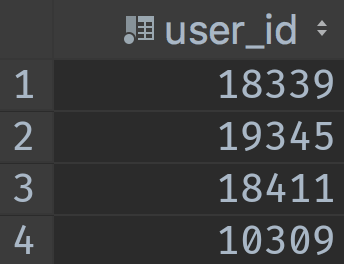
\includegraphics[width=0.15\textwidth]{group.png}
	\caption{Выборка, сформированная \code{group.sql}}
	\label{fig:group}
\end{figure}

\subsection{Добавление записей в таблицы}

В листинге \ref{lst:group.sql} представлен запрос, добавляющий записи во все таблицы.

\lstinputlisting[caption={insert.sql},label={lst:insert.sql}]{insert.sql}

\subsection{Изменение значений полей записей, удовлетворяющих условиям}

В листинге \ref{lst:update.sql} представлен запрос, который в таблице \code{"user"} изменяет логин, равный \code{'null'}, на значение \code{'notnull'}.

\lstinputlisting[caption={update.sql},label={lst:update.sql}]{update.sql}

\subsection{Удаление записей}

В листинге \ref{lst:delete.sql} представлен запрос, который в таблице \code{movie} удаляет все записи, у которых максимальная цена или максимальный рейтинг.

\lstinputlisting[caption={delete.sql},label={lst:delete.sql}]{delete.sql}

В листинге \ref{lst:delete-inner-select.sql} представлен запрос, который в таблице \code{movie} удаляет все записи, для которых в таблице \code{movie\_translation} нет переводов на языки с идентификаторами 1 и 2.

\lstinputlisting[caption={delete-inner-select.sql},label={lst:delete-inner-select.sql}]{delete-inner-select.sql}

\section{Запросы в соответствии с индивидуальным заданием}

\subsection{Запрос 1}

Вывести пользователей, которые смотрят сериалы больше, чем фильмы.

\lstinputlisting[caption={series-lovers.sql},label={lst:series-lovers.sql}]{ind1/series-lovers.sql}

Запрос логически состоит из 3 частей:

\begin{enumerate}
	\item формирование выборки \code{(user\_id, movie\_count)}, в которой каждому пользователю сопоставляется общее количество фильмов, которые он купил, либо которые входят в приобретенные им подписки
	\item формирование выборки \code{(user\_id, episodes\_count)}, в которой каждому пользователю сопоставляется общее число эпизодов сериалов, которые пользователь купил, или которые входят в состав его подписок
	\item соединение двух сформированных выборок и таблицы \code{user}, сравнение для каждого пользователя значений \code{movie\_count} и \code{episodes\_count}, и на основе этого формирование новой выборки для пользователей, у которых значение \code{movie\_count} < \code{episodes\_count}
\end{enumerate}

Первые 5 записей сформированной выборки представлены на рис. \ref{fig:series-lovers}.

\begin{figure}[H]
	\centering
	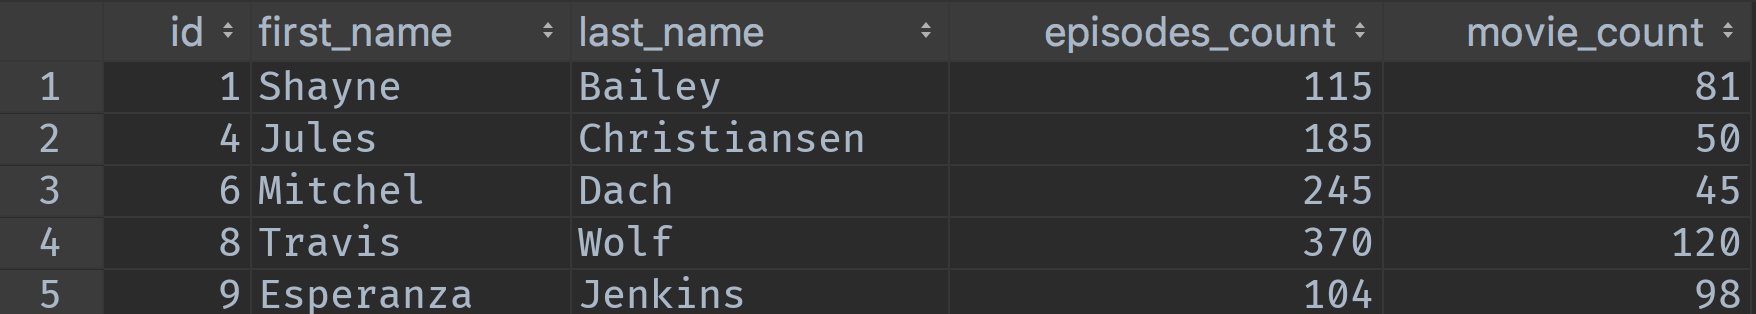
\includegraphics[width=0.8\textwidth]{series-lovers}
	\caption{Выборка, сформированная \code{series-lovers.sql}}
	\label{fig:series-lovers}
\end{figure}

\subsection{Запрос 2}

Вывести сериалы, которые от сезона к сезону увеличивали аудиторию.

\lstinputlisting[caption={series-increasing-audience.sql},label={lst:series-increasing-audience.sql}]{ind2/series-increasing-audience.sql}

Определение того, что от сезона к сезону происходило увеличение аудитории у сериала, сделано следующим образом:

\begin{enumerate}
	\item формируем выборку \code{(series\_id, series\_season\_id, season\_number, audience)} --- идентификатор сериала, идентификатор сезона сериала, номер сезона и аудитория
	\item на основе предыдущей выборки с помощью \code{SELF JOIN} формируем выборку, в которой для каждого сезона сериала, номер которого больше 1, содержится разность аудитории по сравнению с предыдущим сезоном
	\item для каждого сериала считаем количество положительных разностей
	\item если это количество = количеству сезонов в сериале минус 1 (т.к для первого сезона нет предыдущего сезона), то этот сериал нам подходит
\end{enumerate}

Первые 5 записей сформированной выборки представлены на рис. \ref{fig:series-increasing-audience}.

\begin{figure}[H]
	\centering
	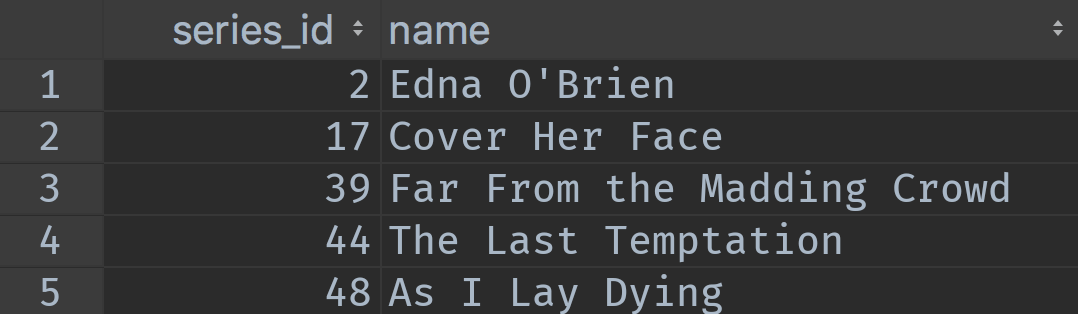
\includegraphics[width=0.4\textwidth]{series-increasing-audience}
	\caption{Выборка, сформированная \code{series-increasing-audience.sql}}
	\label{fig:series-increasing-audience}
\end{figure}

\section{Сохранение в БД выполненных запросов в виде представлений и ХП}

В листинге \ref{lst:views.sql} представлены все ранее написанные \code{SELECT}-запросы в виде представлений.

\lstinputlisting[caption={views.sql},label={lst:views.sql}]{views.sql}

В листинге \ref{lst:stored-procedures.sql} представлены все ранее написанные запросы по добавлению, удалению или обновлению данных в таблицах в виде хранимых процедур.

\lstinputlisting[caption={stored-procedures.sql},label={lst:stored-procedures.sql}]{stored-procedures.sql}

\section{Выводы}

В результате работы был изучен синтаксис языка SQL DML, позволяющий формировать запросы выборки данных из таблиц, формировать запросы по вставке, удалению или обновлению записей в таблицах, создавать на основе запросов представления, которые являются виртуальными таблицами, и создавать хранимые процедуры.

\end{document}
